\documentclass[a4paper, 12pt]{article}
\usepackage[left=1.5cm, text={18cm, 25cm}, top=2.5cm]{geometry}
\usepackage[utf8]{inputenc}
\usepackage[czech,english]{babel}
\usepackage{cite}
\usepackage{graphicx}
\usepackage{float}
\usepackage{amsmath}
\usepackage{amssymb}
\usepackage{tikz}
\usepackage{url}
\usepackage{tikz}
\usepackage{comment}
\usepackage[longend,ruled,vlined,commentsnumbered,linesnumbered]{algorithm2e}
\usepackage{amsthm}
\usepackage{subcaption}

\usetikzlibrary{decorations.pathmorphing}

\newcommand{\myuv}[1]{\quotedblbase #1\textquotedblleft}
\let\oldnl\nl% Store \nl in \oldnl
\newcommand{\nonl}{\renewcommand{\nl}{\let\nl\oldnl}}% Remove line number for one line

\newtheorem{theorem}{Theorem}

\title{Simulation of non-deterministic finite tree automata}
\author{Martin Hruška, Petr Šebek\\\{xhrusk16, xsebek02\}@stud.fit.vutbr.cz}

\date{}
\begin{document}

\maketitle

\section{Introduction}
\label{sec:intro}

\textit{Non-deterministic finite tree automata} (NTA) is a formal model often used in the field of formal verification.
For example, it can be used for shape analysis of the programs manipulating complex data structure where
state of heap is represented by a set of the tree automata \cite{methods12}.
The mentioned technqiue is based on the framework of abstract interpretation where one of the fundamental components
is widening which is done to obtain fixpoint what in this case includes checking inclusion of tree automata languages, i.e.
checking whether language of one NTA is subset of language of the second NTA.
Checking inclusion is easy for deterministic tree automata (DTA) but much harder for NTA because
na{\"i}ve approach requires determinisation of NTA what could lead to exponential growth in the number of the states of NTA.
On the other side, NTA could be exponentially conciser compared to DTA what makes them more suitable for usage in the fields
like formal verification where a state explosion often occurs.
However, there are efficient algorithms for checking language inclusion (based on the antichains \cite{tacas10}) of the NTA.
The antichain based approach could be further imporoved by exploiting \emph{simulation relation} which furher reduce
the number of states of NTA needed to explore during inclusion checking \cite{tacas10}.
On the other side, computation of simulation relation is time consuming itself so the time spend by computing the relation
is sometimes bigger than the time saved by reduction of the number of the visited states.
This leads to need for the new efficient methods for computing simulation to make it fast enough to balance this pay off.
Another usage of simulation is reduction of states NTA which is done by computing equivalence classes on simulation relation and merging states in the same classes.

Efficient algortihm for computing simulation relation has been introduced for finite and infinite graphs \cite{focs95} and
later modified for finite automata in \cite{ilie:nfa} and finally computing simulation for tree automata has been introduced in \cite{tacas08}
where is described computation of either \emph{downward} or \emph{upward} simulation.
Both kinds of the simulations are in \cite{tacas08} computed over labeled transition system (LTS) which is obtained from a NTA.

Mentioned techniques suppose that NTA is represented explicitly what means that their transition relation is not encoded to any special structure but
is saved in e.g. hash tables.
On the other there are techniques dealing with complexity of NTA just by usage of advanced data structures.
One of them is representation of NTA using \textit{mutli-terminal binary decision diagrams} (MTBDD) which are mainly efficient structure for dealing with NTA with large alphabet.
because the symbols of a NTA alphabeth are encoded to binary representation so the transitions can be represented by shared MTBDD in conciser way.
A~NTA could be represented in bottom-up way or top-down way by MTBDD, here we consider only top-down way.

In this work we would like to combine straightforwardness of implementation of simulation over explicitly
represented tree automata and more concise representation of automata by MTBDD.
We suppose NTA represented by MTBDD and we will compute simulation by conversion of MTBDD
to explicit representation with gradual reduction of number of the NTA symbols and also number of transitions.
We use simulation for more efficient language inclusion checking and evaluate whether the method brings any advantage.
The implementation is realized as an extension of VATA library which is state-of-the-art library for NTA manipulation
and contains either implementation of advanced algorithms for inclusion checking and implementation of MTBDD representation of NTA.

The outline of this text is following, in Section \ref{sec:analysis} we give formal definitions, in Section \ref{sec:bdd} MTBDD representation of automata is described.
Section \ref{sec:bdd} describes VATA library, Section \ref{sec:vata} provides description of design of our solution.
Implementation details take place in Section \ref{sec:impl} and finally experiments are evaluated in Section \ref{sec:exps}.

\section{Preliminaries}
\label{sec:analysis}
In this section NTA and simulation over NTA states will be defined more formally.

A~\emph{ranked alphabeth} is a finite set of symbols $\Sigma$ associated with a mapping $\#: \Sigma \rightarrow \mathbb{N}_0$
that assigns ranks to symbols.
Rank of symbol will be also called arity of symbol in following text.
A~\emph{tree} is a graph $t$ which is either empty or it has exactly one root and each of its
nodes is the $i$-th successor of at most one node $v$ for some $i \in \mathbb{N}_0$

A~\emph{finite, non-deterministic, top-down tree automata} is a quadratuple $A=(Q, \Sigma, \delta, R)$ where
$Q$ is a finite set of \emph{states}, $R\subseteq Q$ is a set of \emph{root states}, $\Sigma$ is a ranked alphabeth,
$\delta$ is a set of the transitions.
Each transition is a triple of the form $(q,a,(q_1, \ldots, q_n))$ where $n \geq 0$, $q, q_0 \ldots q_n \in Q$, $a \in \Sigma$ and $\#(a) = n$.
We also denote $(q,a,(q_1, \ldots, q_n))$ as $a(q) \rightarrow (q_1, \ldots, q_n)$.
When $n = 0$ then such a transition is called a \emph{leaf rules}.
A~\emph{bottom-up} automaton is a quadratuple $B=(Q, \Sigma, \delta, F)$, where $Q$, $F$ are same as again set of states and set of final states, $F\subseteq Q$
is a set of final states and $\delta$ is a set of transitions which have the form $(q_1,\ldots, q_n,a,q)$ where $n \geq 0$ and $\#(a) = n$.
We also dennote $(q_1,\ldots, q_n,a,q)$ as $a(q_1, \ldots, q_n) \rightarrow q$.
We can interchange these two notations for non-deterministic tree automata because they have same expressive power in bottom-up and top-down version \cite{tata}.

For a bottom-up NTA $A=(Q, \Sigma, \delta, F)$, a \emph{downward simulation} $\preceq\, \subseteq Q\times Q$ is binary relation such that $q \preceq p$
and $(a(q_1,\ldots, q_n) \rightarrow q) \in \delta$ then $\exists ((p_1, \ldots, p_n) \rightarrow p) \in \delta: \forall i \in {1 \ldots n}: q_i \preceq p_i$.

\section{BDD representation}
\label{sec:bdd}

This section is based on~\cite{fiedor:wsks}. \textit{Reduced ordered binary decision diagram} (ROBDD) is directed acyclic graph with single \textit{source} node called \textit{root} and at least two \textit{sink} nodes 0 and 1. Nodes that are not sink nodes are called \textit{internal nodes}. ROBDD are defined over a set of $n$ Boolean variables $X = \{x_1, \dots, x_n\}$, we assume that $X$ can be ordered: $x_1 < x_2 < \dots < x_n$. Now for each internal node $v$, there exists two outgoing edges with label \textit{low} and \textit{high}. We further can define function \textit{var} which assign Boolean variables to the internal nodes of ROBDD. In ROBDDs there holds next condition: $var(v) < var(v.low) \wedge var(v) < var(v.high) \wedge v.low \neq v.high$, thus successor has always higher value. ROBDD nodes therefore represent $n$-ary Boolean functions that map each assignment to the Boolean variables in $X$.

Mutli-terminal binary decision diagram (MTBDD) is then ROBDD generalized to more than two sink nodes. Further we can define \textit{shared} MTBDD, MTBDD with multiple source nodes/roots. You can see the difference between ordinary BDD and MTBDD in Figure \ref{fig:15860}. %TODO states in right side picture

\begin{figure}[h]
	\centering
	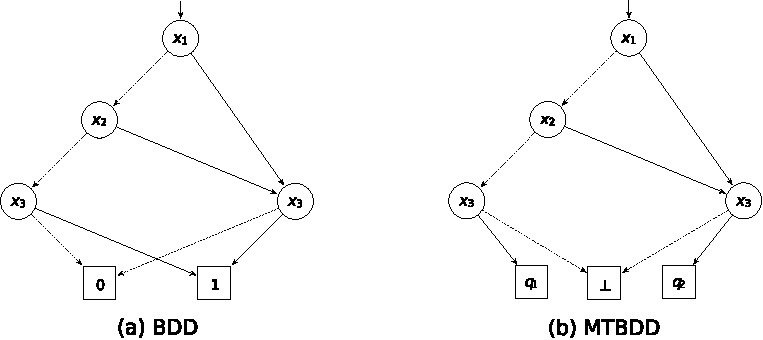
\includegraphics[width=0.7\linewidth]{15860.pdf}
	\caption{Comparison of ROBDD and MTBDD \cite{fiedor:wsks}}
	\label{fig:15860}
\end{figure}

Let $A=(Q, \Sigma, \delta, R)$ be a tree automaton. We can encode symbols to binary sequence with some function $enc: \Sigma \rightarrow \{0, 1\}^n$, for some $n$. Each position $1\leq i \leq n$ is then assigned a Boolean variable from set $X = \{x_1, \dots, x_n\}$. We define $Q^\#$ as set of all tuples of states from $Q$ with up to the maximum arity that some symbol in $\Sigma$ has.

Finally we can define \textit{top-down} representation of the transition function $\delta$ of the TA $A$ uses a shared MTBDD $\delta^{td}$ over $\Sigma$, where the set of roots $R=Q$ and the domain of labels of sink nodes is $2^{Q^\#}$. MTBDD $\delta^{td}$ then represents the function
\begin{equation*}
[[ \delta^{td}]]  : Q \rightarrow (\Sigma \rightarrow 2^{Q^\#}t)
\end{equation*}
\begin{equation*}
[[ \delta^{td}]]   = \lambda q a . \{(q_1, \dots, q_p) | q \xrightarrow{a} (q_1, \dots, q_p) \} 
\end{equation*}

As an example we can take top-down TA with following transitions:
\begin{alignat*}{4}
q_1 \xrightarrow{00\overline{X}} q_1, \qquad &
q_1 \xrightarrow{011} q_1, \qquad & 
q_1 \xrightarrow{110} q_1, \qquad &
q_1 \xrightarrow{10\overline{X}} q_1, \qquad & \\
q_1 \xrightarrow{010} q_1, \qquad &
q_1 \xrightarrow{111} q_1, \qquad &
q_1 \xrightarrow{\overline{X}\overline{X}\overline{X}} q_2 \qquad &  &\\
\end{alignat*}

Where symbol $\overline{X}$ denotes either 0 or 1. MTBDD encoding this transition is depicted at Figure~\ref{fig:MTBDD}.

\begin{figure}[h]
\centering
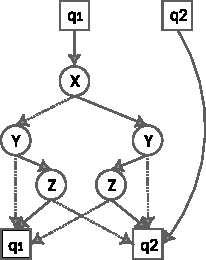
\includegraphics[width=4cm]{MTBDD}
\caption{Example of MTBDD representing automaton transitions \cite{fiedor:wsks}}
\label{fig:MTBDD}
\end{figure}


\section{VATA}
\label{sec:vata}
VATA is library for efficient manipulation with NTA \cite{libvata}.
It provides both encodings of NTA -- semi-symbolic via MTBDD and explicit which will be described further.
VATA is open-source licensed under GPL license and it is written in C++. You can see internal library design in Figure~\ref{fig:lib_design}.
It currently supports TIMBUK as input format. 

The main goal of VATA is to provide state-of-the-art algorithms for inclusion checking
but it also contains implementation of standard operations like union or intersection of languages of NTA.
As we mentioned in Section \ref{sec:intro} inclusion checking is related to simulation
since simulation relation could bring more efficiency to the state-of-the-art algorithms like antichains \cite{tacas10}.
There are already implemented algorithms for computing simulation in VATA.
The algorithms for simulation computing in VATA uses computation over LTL systems from \cite{tacas08} for explicit encoding
and there are also some na{\"i}ve implementations for bottom-up MTBDD.

\begin{figure}[h]
	\centering
	\begin{tikzpicture}
[
  scale=0.85,
  transform shape,
	gen/.style={thick,fill=gray!10},
	expl/.style={thick,fill=orange!50},
	bu/.style={thick,fill=green!40},
	td/.style={thick,fill=blue!30},
	other/.style={fill=yellow!10,dashed}
]

% encodings
\draw[dashed] (0,1) -- (-1.7,2.5);
\draw[dashed] (0,0) -- (-1.7,1.5);
\draw[dashed] (3,1) -- (1.3,2.5);

\draw (0,0.5) rectangle +(3, 0.5) [gen] node[midway] {\textit{\scriptsize{Encoding}}};
\draw (0,0) rectangle +(1.3, 0.5) [gen] node[midway] {\textit{\scriptsize{Core}}};
\draw (1.3,0) rectangle +(1.7, 0.5) [gen] node[midway] {\textit{\scriptsize{Operations}}};

\draw (-5.1,2) rectangle +(3, 0.5) [expl] node[midway] {\scriptsize{Explicit}};
\draw (-5.1,1.5) rectangle +(1.3, 0.5) [expl] node[midway] {\scriptsize{Core}};
\draw (-3.8,1.5) rectangle +(1.7, 0.5) [expl] node[midway] {\scriptsize{Operations}};

\draw (-1.7,2) rectangle +(3, 0.5) [bu] node[midway] {\scriptsize{MTBDD Bottom-Up}};
\draw (-1.7,1.5) rectangle +(1.3, 0.5) [bu] node[midway] {\scriptsize{Core}};
\draw (-0.4,1.5) rectangle +(1.7, 0.5) [bu] node[midway] {\scriptsize{Operations}};

\draw (1.7,2) rectangle +(3, 0.5) [td] node[midway] {\scriptsize{MTBDD Top-Down}};
\draw (1.7,1.5) rectangle +(1.3, 0.5) [td] node[midway] {\scriptsize{Core}};
\draw (3.0,1.5) rectangle +(1.7, 0.5) [td] node[midway] {\scriptsize{Operations}};

\draw (5.1,2) rectangle +(3, 0.5) [other] node[midway] {\scriptsize{$<$other$>$}};
\draw (5.1,1.5) rectangle +(1.3, 0.5) [other] node[midway] {\scriptsize{Core}};
\draw (6.4,1.5) rectangle +(1.7, 0.5) [other] node[midway] {\scriptsize{Operations}};

\draw[dashed] (3,0) -- (1.3,1.5);

\draw[rounded corners=9,dash pattern=on 3pt off 2pt on 1pt off 2pt] (-5.5,-0.5) rectangle +(14,3.4);

\draw (6.6,0) node {\textit{Automata encodings}};


% parsers
\draw (-5,-2) rectangle +(3, 1) [gen,fill=brown!40] node[midway] (parser1) {\textit{Parser1}};
\draw (-5,-3.5) rectangle +(3, 1) [gen,fill=brown!40] node[midway] {\textit{Parser2}};
\draw (-3.5,-4) node {$\vdots$};

\draw[rounded corners=9,dash pattern=on 3pt off 2pt on 1pt off 2pt] (-5.5,-0.7) rectangle +(4.1,-4);
\draw (-2.3,-4.2) node {\textit{Parsers}};

% serializers
\draw (5,-2) rectangle +(3, 1) [gen,fill=brown!40] node[midway] {\textit{Serializer1}};
\draw (5,-3.5) rectangle +(3, 1) [gen,fill=brown!40] node[midway] {\textit{Serializer2}};
\draw (6.4,-4) node {$\vdots$};

\draw[rounded corners=9,dash pattern=on 3pt off 2pt on 1pt off 2pt] (4.4,-0.7) rectangle +(4.1,-4);
\draw (7.5,-4.2) node {\textit{Serializers}};

% program
\draw[rounded corners=9,dash pattern=on 3pt off 2pt on 1pt off 2pt] (-1.2,-0.7) rectangle +(5.4,-4);

\draw[fill=olive!60] (-0.6,-1.5) rectangle (3.6,-3.5) node[midway] {\textit{Program}};

\draw[very thick,dashed,->,black!70] (-0.6,-1.7) -- (-2,-1.7);
\draw[very thick,dashed,->,black!70] (3.6,-3) -- (5,-3);
\draw[very thick,dashed,->,black!70] (0.8,-1.5) -- (0.8,0);
\draw[very thick,dashed,->,black!70] (2.2,-1.5) -- (2.2,0);

\end{tikzpicture}

	\caption{VATA library design. Image is taken from \cite{libvata}.}
	\label{fig:lib_design}
\end{figure}

\begin{figure}[h]
	\centering
	\begin{tikzpicture}
[
  scale=0.85,
  transform shape,
	gen/.style={thick,fill=gray!10},
	expl/.style={thick,fill=orange!50},
	bu/.style={thick,fill=green!40},
	td/.style={thick,fill=blue!30},
	other/.style={fill=yellow!10,dashed}
]

\node at(10,2) {Automata};

\node[expl,circle,draw] (aA) at(1.25,2) {\textit{$A$}};
\node[expl,circle,draw] (aB) at(3.75,2) {\textit{$B$}};
\node[expl,circle,draw] (aC) at(6.25,2) {\textit{$C$}};


\node at(10,0) {\shortstack{Top-level\\ Lookup Tables}};

\node[minimum size=40pt](table1) at (2.75,0) {};
\draw (2,0) rectangle +(0.5, .5) [td] node[midway] {\textit{$q_1$}};
\draw (2,-.5) rectangle +(0.5, .5) [td] node[midway] {};
\draw (2.5,0) rectangle +(0.5, .5) [td] node[midway] {\textit{$q_2$}};
\draw (2.5,-.5) rectangle +(0.5, .5) [td] node[midway] {};
\draw (3,0) rectangle +(0.5, .5) [td] node[midway] {\textit{$q_3$}};
\draw (3,-.5) rectangle +(0.5, .5) [td] node[midway] {};

\node[minimum size=40pt](table2) at (5,0) {};
\draw (4.5,0) rectangle +(0.5, .5) [td] node[midway] {\textit{$q_1$}};
\draw (4.5,-.5) rectangle +(0.5, .5) [td] node[midway] {};
\draw (5,0) rectangle +(0.5, .5) [td] node[midway] {\textit{$q_2$}};
\draw (5,-.5) rectangle +(0.5, .5) [td] node[midway] {};


\draw[->,thick,dashed] (aA) -- (table1);
\draw[->,thick,dashed] (aB) -- (table2);
\draw[->,thick,dashed] (aC) -- (table2);


\node at(10,-2) {Transition Clusters};

\node[minimum size=35](cluster1) at (1.5,-2) {};
\draw (0.75,-2) rectangle +(0.5, .5) [td] node[midway] {\textit{$a$}};
\draw (0.75,-2.5) rectangle +(0.5, .5) [td] node[midway] {};
\draw (1.25,-2) rectangle +(0.5, .5) [td] node[midway] {\textit{$b$}};
\draw (1.25,-2.5) rectangle +(0.5, .5) [td] node[midway] {};

\node[minimum size=35pt](cluster2) at (3.25,-2) {};
\draw (2.75,-2) rectangle +(0.5, .5) [td] node[midway] {\textit{$c$}};
\draw (2.75,-2.5) rectangle +(0.5, .5) [td] node[midway] {};
\draw (3.25,-2) rectangle +(0.5, .5) [td] node[midway] {\textit{$e$}};
\draw (3.25,-2.5) rectangle +(0.5, .5) [td] node[midway] {};

\node[minimum size=35pt](cluster3) at (5.25,-2) {};
\draw (4.75,-2) rectangle +(0.5, .5) [td] node[midway] {\textit{$b$}};
\draw (4.75,-2.5) rectangle +(0.5, .5) [td] node[midway] {};
\draw (5.25,-2) rectangle +(0.5, .5) [td] node[midway] {\textit{$c$}};
\draw (5.25,-2.5) rectangle +(0.5, .5) [td] node[midway] {};

\node[minimum size=35pt](cluster4) at (6.5,-2) {};
\draw (6.25,-2) rectangle +(0.5, .5) [td] node[midway] {\textit{$e$}};
\draw (6.25,-2.5) rectangle +(0.5, .5) [td] node[midway] {};


\draw[thick,fill=black] (2.25,-0.25) circle (0.5mm);
\draw[->,thick,dashed] (2.25,-.25) -- (cluster2);

\draw[thick,fill=black] (2.75,-0.25) circle (0.5mm);
\draw[->,thick,dashed] (2.75,-.25) -- (cluster1);

\draw[thick,fill=black] (3.25,-0.25) circle (0.5mm);
\draw[->,thick,dashed] (3.25,-.25) -- (cluster3);

\draw[thick,fill=black] (4.75,-0.25) circle (0.5mm);
\draw[->,thick,dashed] (4.75,-.25) -- (cluster2);

\draw[thick,fill=black] (5.25,-0.25) circle (0.5mm);
\draw[->,thick,dashed] (5.25,-.25) -- (cluster4);


\node at(10,-3.75) {\shortstack{Sets of\\ Pointers to Tuples}};

\node[minimum size=25pt](set1) at (0.25,-3.75) {};
\draw (0,-4) rectangle +(0.5, .5) [td] node[midway] {};

\node[minimum size=25pt](set2) at (1.5,-3.75) {};
\draw (1,-4) rectangle +(0.5, .5) [td] node[midway] {};
\draw (1.5,-4) rectangle +(0.5, .5) [td] node[midway] {};

\node[minimum size=25pt](set3) at (2.75,-3.75) {};
\draw (2.5,-4) rectangle +(0.5, .5) [td] node[midway] {};

\node[minimum size=25pt](set4) at (3.75,-3.75) {};
\draw (3.5,-4) rectangle +(0.5, .5) [td] node[midway] {};

\node[minimum size=25pt](set5) at (4.75,-3.75) {};
\draw (4.5,-4) rectangle +(0.5, .5) [td] node[midway] {};

\node[minimum size=25pt](set6) at (6,-3.75) {};
\draw (5.5,-4) rectangle +(0.5, .5) [td] node[midway] {};
\draw (6,-4) rectangle +(0.5, .5) [td] node[midway] {};

\node[minimum size=25pt](set7) at (7.25,-3.75) {};
\draw (7,-4) rectangle +(0.5, .5) [td] node[midway] {};


\draw[thick,fill=black] (1,-2.25) circle (0.5mm);
\draw[->,thick,dashed] (1,-2.25) -- (set1);

\draw[thick,fill=black] (1.5,-2.25) circle (0.5mm);
\draw[->,thick,dashed] (1.5,-2.25) -- (set2);

\draw[thick,fill=black] (3,-2.25) circle (0.5mm);
\draw[->,thick,dashed] (3,-2.25) -- (set3);

\draw[thick,fill=black] (3.5,-2.25) circle (0.5mm);
\draw[->,thick,dashed] (3.5,-2.25) -- (set4);

\draw[thick,fill=black] (5,-2.25) circle (0.5mm);
\draw[->,thick,dashed] (5,-2.25) -- (set5);

\draw[thick,fill=black] (5.5,-2.25) circle (0.5mm);
\draw[->,thick,dashed] (5.5,-2.25) -- (set6);

\draw[thick,fill=black] (6.5,-2.25) circle (0.5mm);
\draw[->,thick,dashed] (6.5,-2.25) -- (set7);


\node at(10,-5.5) {Tuples of States};

\node(tup1) at (0.75,-5.5) {$(q_1, q_1)$};
\node(tup2) at (2.5,-5.5) {$(q_1, q_2)$};
\node(tup3) at (4.25,-5.5) {$(q_2, q_2)$};
\node(tup4) at (7,-5.5) {$(q_3, q_2)$};
\node(tup5) at (5.5,-5.5) {$()$};

\draw[thick,fill=black] (0.25,-3.75) circle (0.5mm);
\draw[->,thick,dashed] (0.25,-3.75) -- (tup1);

\draw[thick,fill=black] (1.25,-3.75) circle (0.5mm);
\draw[->,thick,dashed] (1.25,-3.75) -- (tup1);

\draw[thick,fill=black] (1.75,-3.75) circle (0.5mm);
\draw[->,thick,dashed] (1.75,-3.75) -- (tup2);

\draw[thick,fill=black] (2.75,-3.75) circle (0.5mm);
\draw[->,thick,dashed] (2.75,-3.75) -- (tup2);

\draw[thick,fill=black] (3.75,-3.75) circle (0.5mm);
\draw[->,thick,dashed] (3.75,-3.75) -- (tup5);

\draw[thick,fill=black] (4.75,-3.75) circle (0.5mm);
\draw[->,thick,dashed] (4.75,-3.75) -- (tup2);

\draw[thick,fill=black] (5.75,-3.75) circle (0.5mm);
\draw[->,thick,dashed] (5.75,-3.75) -- (tup3);

\draw[thick,fill=black] (6.25,-3.75) circle (0.5mm);
\draw[->,thick,dashed] (6.25,-3.75) -- (tup4);

\draw[thick,fill=black] (7.25,-3.75) circle (0.5mm);
\draw[->,thick,dashed] (7.25,-3.75) -- (tup5);


\end{tikzpicture}

	\caption{Explicit representation of automaton. Image is taken from \cite{libvata}.}
	\label{fig:explicit}
\end{figure}

\begingroup
\tikzset{every picture/.style={scale=1.3}}%
\begin{figure}[h]
	\centering
	\begin{subfigure}{.5\textwidth}
		\centering
		\begin{tikzpicture}
[]
\useasboundingbox (-2.9,-4.9) rectangle (2.7,0.6);

<<<<<<< HEAD
=======

>>>>>>> fcad047018e021c44f6be41eab656d5ec3da0ca5
%\draw[thick,fill=blue!40] (3,-5) -- (0,0) -- (-3,-5) .. controls (-1,-3.5) and (1,-6.5) .. (3,-5);
\draw[thick,fill=pink] (2,-3.5) -- (0,0) -- (-2,-3.5) decorate[decoration=snake,segment length=22] { -- cycle};

\node at (0,0.4){$q$};

\node(set1) at (-2,-4.2) {$\{(r,s),(r, t)\}$};
\node(set2) at (-0.5,-4.7) {$\{(s), (t), (u)\}$};
\node(set3) at (0.8,-4.2) {$\emptyset$};
\node(set4) at (2,-4.5) {$\{(u, u, u)\}$};

\draw[->,thick,dashed,rounded corners] (-0.05,-0.2) -- (-0.35,-1.2) -- (-1,-1.9) -- (-1,-2.5) -- (-1.4,-2.8) -- (set1);
\draw[->,thick,dashed,rounded corners] (-0.02,-0.3) -- (0,-1) -- (-0.6,-1.9) -- (0,-2.3) -- (-0.5,-2.5) -- (-1,-2.8) -- (set2);
\draw[->,thick,dashed,rounded corners] (0.02,-0.3) -- (0.35,-1.8) -- (0.5,-2.75) -- (1.3,-3) -- (set3);
\draw[->,thick,dashed,rounded corners] (0.05,-0.2) -- (0.6,-1.5) -- (1,-1.9) -- (0.9,-2.7) -- (1.5,-2.8) -- (set4);



\end{tikzpicture}
		\caption{MTBDD Top-down. Image is taken from \cite{libvata}.}
		\label{fig:mtbdd_td}
	\end{subfigure}%
	~
	\begin{subfigure}{.5\textwidth}
	\centering
	\begin{tikzpicture}
[]
\useasboundingbox (-2.9,-4.9) rectangle (2.7,0.6);
\draw[thick,fill=blue!40] (3,-5) -- (0,0) -- (-3,-5) .. controls (-1,-3.5) and (1,-6.5) .. (3,-5);
%\draw[thick,fill=blue!40] (2,-3.5) -- (0,0) -- (-2,-3.5) decorate[decoration=snake,segment length=22] { -- cycle};

\node at (0,0.4){$(q_1,\dots, q_n)$};

\node(set1) at (-2,-4.2) {$\{r,s\}$};
\node(set2) at (-0.5,-4.4) {$\{s, t, u\}$};
\node(set3) at (0.8,-4.2) {$\emptyset$};
\node(set4) at (2,-4.4) {$\{u\}$};

\draw[->,thick,dashed,rounded corners] (-0.05,-0.2) -- (-0.35,-1.2) -- (-1,-1.9) -- (-1,-2.5) -- (-1.4,-2.8) -- (set1);
\draw[->,thick,dashed,rounded corners] (-0.02,-0.3) -- (0,-1) -- (-0.6,-1.9) -- (0,-2.3) -- (-0.5,-2.5) -- (-1,-2.8) -- (set2);
\draw[->,thick,dashed,rounded corners] (0.02,-0.3) -- (0.35,-1.8) -- (0.5,-2.75) -- (1.3,-3) -- (set3);
\draw[->,thick,dashed,rounded corners] (0.05,-0.2) -- (0.6,-1.5) -- (1,-1.9) -- (0.9,-2.7) -- (1.5,-2.8) -- (set4);



\end{tikzpicture}
	\caption{MTBDD Bottom-up. Image is taken from \cite{libvata}.}
	\label{fig:mtbdd_bu}
	\end{subfigure}%
\end{figure}
\endgroup

\subsection{Explicit representation}

Let consider transitions in form $a(q_1,\ldots,q_n) \rightarrow q$.
The explicitly represented automata transition set is implemented using two hash maps.
The first one, called \emph{Top-level Lookup Tables}, maps each state (e.g. $q$) to it \emph{Transition cluster}.
Transition cluster then maps symbols (e.g. $a$) to \emph{sets of pointers to tuples}.
Pointers to tuples finally reference to storage of the tuples (e.g. $a(q_1,\ldots,q_n) \rightarrow q$).
Explicit representation is depicted in Figure~\ref{fig:explicit}.
The set of states is not stored explicitly because it is possible to obtain it from transition relation.
However, a set of final states is represented like a standard set.

\subsection{Semi-Symbolic Representation}

Semi-symbolic representation is based on representing transition relation using MTBDD.
The particular details of encoding of a NTA to MTBDD is described in section \ref{sec:bdd}.
The VATA library provides two possible MTBDD representation -- top-down and bottom-up. These two types are depicted in Figures~\ref{fig:mtbdd_td} and \ref{fig:mtbdd_bu}. 
The first one stores MTBDD for each $q \in Q$ of NTA $A=(Q,\Sigma, \delta, F)$ and all transition where $q$ is on right-handed side
are represented by the MTBDD.
The MTBDD terminal symbols are sets of tuples which it is possible to make transition from $q$ to under a symbol from $\Sigma$.
The bottom-up representation is inverse, MTBDD exists for each tuple of the NTA and it represents all transitions with
the tuple on the left-handed side and the terminal symbols are sets of states which it is possible to make transition to from the tuple.

\section{Design}
\label{sec:design}

This section describes conceptual design of our method for computing simulation.
For implementation details please see Section \ref{sec:impl}.

As the input of our method we take a NTA represented by MTBDD in top-down way
which we translate into a NTA represented explicitly and we also reduce number of the symbols.
Simulation relation is finally computed over the explicit NTA.
The mentioned conversion is done by following general method for reduction of alphabet and yielding a new NTA.
Let have a NTA $A=(Q, \Sigma, \delta, F)$, a new ranking alphabet $\Sigma'$ and mapping $f: 2^\Sigma \rightarrow \Sigma'$,
when there is $((a_1(q_1,\ldots,q_n) \rightarrow q) \in \delta \wedge \ldots \wedge (a_m(q_1,\ldots,q_n) \rightarrow q) \in \delta) \wedge
((a_1(r_1,\ldots,r_n) \rightarrow q) \in \delta \wedge \ldots \wedge (a_n(r_1,\ldots,r_n) \rightarrow q) \in \delta)$
such that $a_i \neq a_{i+1}$ for any $i\in \{1..n\}$ then if $f(\{a_1,\ldots, a_n\} = \emptyset$ do $\Sigma' = \Sigma' \cup X$ such that $X \notin \Sigma'$
and add $(\{a_1, \ldots, a_n\}) \rightarrow X)$ to $f$.
There is also constructed a new NTA $A' = (Q, \Sigma', \delta', F)$ where $Q, F$ are unchanged to $A$ 
and $\Sigma'$ is the new ranked alphabeth obtained by mapping $f$ and $\delta'$ is transition set such that
if $(a_1(q_1, \ldots, q_n) \rightarrow q) \in \delta \wedge \ldots \wedge (a_n(q_1, \ldots, q_n) \rightarrow q) \in \delta$ and
$ (\{a_1,\ldots,a_n\}  \rightarrow X)~\in f$ for some $X \in \Sigma'$, then $(X(q_1, \ldots, q_n) \rightarrow q) \in \delta'$
for all possible tuples $q_1,\ldots,q_n$.

In our case, the input of the mentioned method NTA is semi-symbolic represented one and the output NTA is the same automata in explicit representation.
The transformation of NTA representation is done in level of implementation details and it is not directly related to a design of generic algorithm.
The whole method of translation is described algorithmcally in Algortihm \ref{alg:translate}.

\begin{algorithm}[h]
\KwIn{NTA $A=(Q,\Sigma, \delta, F)$}
    \KwOut{NTA $A'=(Q,\Sigma', \delta', F)$}
    $\delta' := \emptyset $\;
    $\Sigma' := \emptyset $\;
	$f := \emptyset$\;
	\ForEach{$q \in Q$}
    {
		\ForEach{$(q_1,\ldots, q_n)$, such that $(a(q_1, \ldots, q_n)\rightarrow q) \in \delta)$ for any $a\in \Sigma$}
		{
			$S_q := \{ a\in \Sigma \,|\, \exists(a(q_1,\ldots,q_n) \rightarrow q) \in \delta\}$\;
			\ForEach{$(r_1,\ldots, r_n)$, such that $(b(r_1, \ldots, r_n)\rightarrow q) \in \delta)$ for any $a\in \Sigma$}
			{
				$S_r := \{a\in \Sigma \,|\, \exists\, (a(r_1,\ldots,r_n) \rightarrow q) \in \delta\}$\;
				\If{$(S_q \cap S_r \rightarrow A') \not\in f$ for any $A' \in \Sigma'$}
				{
					add $A'$ to $\Sigma'$ such that $A' \not\in \Sigma'$\;
					add $(S_q \cap S_r \rightarrow A')$ to $f$\;
				}
				add $f(S_q \cap S_r)(q_1,\ldots,) \rightarrow q$ to $\delta'$\;
			}
		}
    }
	\Return $A' = (Q, \Sigma', \delta', F)$
\caption{NTA symbol reduction yielding a new NTA}
\label{alg:translate}
\end{algorithm}


\begin{theorem}
Let have a NFA $A = (Q, \Sigma, \delta, F)$ and $n = |Q|$, $m = |\delta|$ and let also ignore implementation
complexity of the used data structures.
Complexity of Algorithm \ref{alg:translate} is $O(m^2)$.
\end{theorem}
\begin{proof}
Initialization at lines $1-3$ has constant complexity $O(3)$.
The number of the iterations of the cycles at lines $4,5$ is at most $O(m)$ times because for each state $q\in Q$ (line 4) are
visited all transitions where $q$ is at right-handed side.
Complexity of operation at line $6$ is $O(1)$.
Cycle at line $7$ is iterated at most $O(m)$ (when it go through all transitions).
The line $8-12$ are $O(5)$ (here we ignore implementation details).
Putting all together we have following complexity: $O(3) + O(m)*(O(u)+O(m)*O(v)) = O(m*u + m^2+v)$
\end{proof}

When explicitly represented automata is obtained it is possible to compute simulation using standard algorithm.
First, we tried the algorithm described in \ref{lengal:trees} which is na{\"i}ve one and is described in Algorithm \ref{alg:sim}.

\begin{algorithm}[h]
\KwIn{NTA $A=(Q,\Sigma, \delta, F)$}
	\KwOut{$\preceq \subseteq Q \times Q$}
	\SetKwFunction{main}{main}
	\SetKwProg{main}{}{}{}
    
	$last := \emptyset $\;
    $sim := \emptyset $\;
	\While{$sim \neq last$}
	{
		$last := sim$\;
		\ForEach{Arity $n$ of $\Sigma$}
		{
			\ForEach{$a \in \Sigma$ such that $\#(a) = n$}
			{
				\ForEach{$(q_1,\ldots, q_n)$, such that $(a(q_1, \ldots, q_n)\rightarrow q) \in \delta)$ for any $q \in Q$}
				{
					$temp := \emptyset$\;
					\ForEach{$(r_1,\ldots, r_n)$, such that $(a(r_1, \ldots, r_n)\rightarrow r) \in \delta)$ for any $r \in Q$ and 
					$q_1 \preceq r_1 \wedge \ldots \wedge q_n \preceq r_n$}
					{
						$temp := temp \cup \{r \in Q \,|\, a(r_1,\ldots, r_n) \rightarrow r\}$\;
					}

					$simRefiment(sim, \{q \in Q \,|\, a(q_1,\ldots, q_n) \rightarrow q\}, temp)$\;
				}
			}
		}

	}
	\Return $sim$\;
	\DontPrintSemicolon \nonl\;
	\setcounter{AlgoLine}{0}

	\SetKwFunction{simRefiment}{simRefiment}
	\SetKwProg{refProc}{Function}{}{}
	\nonl \refProc{\simRefiment{$sim$,$lhs$,$rhs$}}
	{
		\ForEach{$q \in lhs$}
		{
			\ForEach{$(q,r) \in sims$}
			{
				\If{$r \notin rhs$}
				{
					remove $(q,r)$ from $sim$ \;
				}
			}
		}
	 }
	 \caption{Computing simulation on a NTA. The algorithm is based on the one in \cite{lengal:trees}}
\label{alg:sim}
\end{algorithm}

\begin{theorem}
	\label{the:nfacompl}
Let have a NTA $A = (Q, \Sigma, \delta, F)$ and let $n = |Q|$, $m = |\delta|$.
Complexity of Algorithm \ref{alg:sim} is $O(m^2*n^4)$
\end{theorem}

\begin{proof}
	The lines $1-2$ in main function of Algorithm \ref{alg:sim} takes constant time $O(1)$.
	Cycle beginning at line $3$ will be repeated at most $n^2$ because $sim$ is initialized with size $n^2$
	and at the worst case it is possible that its items are removed gradually in iteration one by one.
	The cycles at lines $5-7$ has complexity $O(m)$ since we iterate over all arities $n$ and over all symbols $a$ with arity $n$
	and over all transitions symbol $a$ so we iterate over all transitions.
	Line $8$ takes again constant time $O(1)$.
	Cycle at line $9$ has complexity $O(m)$ because in the worst case there is only one symbol with one arity.
	so this cycle will iterate over all transitions again.
	Complexity of line $10$ is constant $O(1)$.
	Function $simRefiment$ has complexity $O(n^2)$ because it could iterate over each element of $sim$ what could be $O(n^2)$.
	Removing items from $sim$ at line $4$ have constant complexity so it does not change anything at all.
	Taking all together, Algorithm \ref{alg:sim} has following complexity 
	$O(2) + O(n^2)*(O(m)*(1+O(m)+O(n^2)))=
	O(2) + O(n^2)*(O(m)+O(m^2)+O(m^2*n^2)) =
	O(n^2)*(O(m^2*n^2)) =
	O(m^2*n^4)$
\end{proof}

Theorem \ref{the:nfacompl} shows that complexity of Algorithm \ref{alg:sim} is very high what leads us
to modify algortihm for simulation computation over NTA from \cite{ilie:nta}.
This algorithm is designed for nondeterministic finite automata so it was neccessary to modify it for NTA.
We propose such a modification in Algorithm \ref{alg:sim1}.

\begin{algorithm}[h]
	\KwIn{NTA $A=(Q,\Sigma, \delta, F)$}
	\KwOut{$\preceq \subseteq Q \times Q$}
	\SetKwFunction{main}{main}
	\SetKwProg{main}{}{}{}

	\ForEach{$q\in Q$} {
		\ForEach{$a\in \Sigma$} {
			$\delta^r(q,a) = \{k \in Q\,|\, a(q_1,\ldots, q_i, \ldots, q_n) \rightarrow k \emph{ where } i \in \{1..n\}, q = q_i \}$\;
			$card(q,a) = |\{a(q_1, \ldots, q_n) \rightarrow q \in \delta\}|$\;
		}
	}

	initialize all $N(a)$s with $0$s\;
	$sim := Q\times Q$\;
	$C := \emptyset$\;

	\ForEach{$p \in F$} {
		\ForEach{$q \in Q \setminus F$} {
			$sim = sim \setminus \{(p,q)\}$\;
			$C = C \cup \{(p,q)\}$\;
		}
	}
	
	\While{$C \neq \emptyset$}
	{
		Take $(p,q)$ from $C$\;
		\ForEach{$a \in \Sigma$}
		{
			\ForEach{$k \in \delta^r(q,a)$}
			{
				\If {$(a(q_1,\ldots, q_i, \ldots, q_n) \rightarrow k) \in \delta \wedge
					(a(p_1, \ldots, p_i, \ldots, p_n) \rightarrow p') \in \delta, \emph{ where } i\in \{1..n\},\ q_i = q,\ p_i = p $}
				{
					$N_{kp}(a) = N_{kp}(a) + 1$\;
				}

				\If{$N_{kp}(a) = card(k,a)$}
				{
					\ForEach{$l \in \delta^r(p,a)$}
					{
						\If{$(l,k) \in sim$}
						{
							$sim = sim \setminus {(l,k)}$\;
							$C = C \cup {(l,k)}$\;
						}
					}
				}
			}
		}

	}
	\Return $sim$\;

	 \caption{Computing simulation on a NTA efficiently. Based on similiar algortihm for finite automata in \cite{ilie:nfa}.}
\label{alg:sim1}
\end{algorithm}

The whole complexity of our method is $O(m^2)+O(m^2*n^4)$.
As you mentiond we ignore complexity of manipulation of the used data structures.
We know that this could changed the complexity of the algorithms in practice but the proofs would be much more complex in that case
and we would like to show complexity related to the number of the states and size of transition relation in more abstract way.

\section{Implementation}
\label{sec:impl}

As we mentioned in Section \ref{sec:vata} VATA library already has infrastructure needed for implementation of
our method.
It contains support for parsing input NTA, its semi-symbolic and explicit representation and implemented
state-of-the-art algorithm for inclusion checking so we decided to implement our solution as extension of VATA library.
We design our implementation like a stand-alone module which is compiled separately to the rest of library (using CMake building system).
Our module needs just include some headers for knowing interface of VATA classes for NTA representation.

Being more specific, our module is consisted from the following classes related to design proposed in Section \ref{sec:design}
\begin{itemize}
	\item \emph{BDDTopDownSimExpl} Class translates MTBDD represented automaton to explicit one with symbol translation using Algorithm \ref{alg:transl}.
	\item \emph{BDDTopDownSimComputer} Class computes downward simulation over explicit tree automata using Algorithm \ref{alg:sim}.
	\item \emph{BDDTopDownSimEfficient} Class computes downward simulation over explicit tree automata using Algorithm \ref{alg:sim1}.
	\item \emph{Supporting data types} Supporting data types and fuctions for previous classes are included in the following files \emph{data\_types.hh, sim\_efficient\_types.hh, sim\_efficient\_types\_functor.hh}
\end{itemize}

We exploited following classes from VATA implementation:

\begin{itemize}
	\item \emph{BDDTDTreeAutCore} Class for semi-symbolic representation of NTA using MTBDD.
	\item \emph{ExplicitTreeAutCore} Class for explicit representation of NTA.
	\item \emph{BinaryDiscontRelation} Class for representation of simulation relation.
\end{itemize}

\section{Experiments}
\label{sec:exps}

The experiments should find out how big efficiency brings our method for computing simulation for checking inclusion of the tree automata.
The experiments was done by checking inclusion of language each automaton to other automata with and without simulation
and comparing needed times for checking inclusion depending on the number of states of the automata.
The time for computing simulation was included into the time needed for checking inclusion with simulation
because it is not often possible to reuse once computed simulation.

We ran experiments on automata from VATA test folder. First we ran experiment with automata with number of states from range 0-60. You can see result of this experiment in Figure~\ref{fig:g}. Please note that y axis is in logarithmic scale. Also note that plots are sorted by nosim\_time, run without simulation. Our experiments had timeout 60 seconds. We checked if result of inclusion with simulation correspond with result of run without simulation. We have 100 \% success rate in computing inclusion result, therefore our simulation algorithm is implemented correctly.

All experiments were ran on computer with OS Fedora 20 with CPU Intel Core i5-2520M with available 8 GiB of RAM.

\begin{figure}[h!]
	\centering
	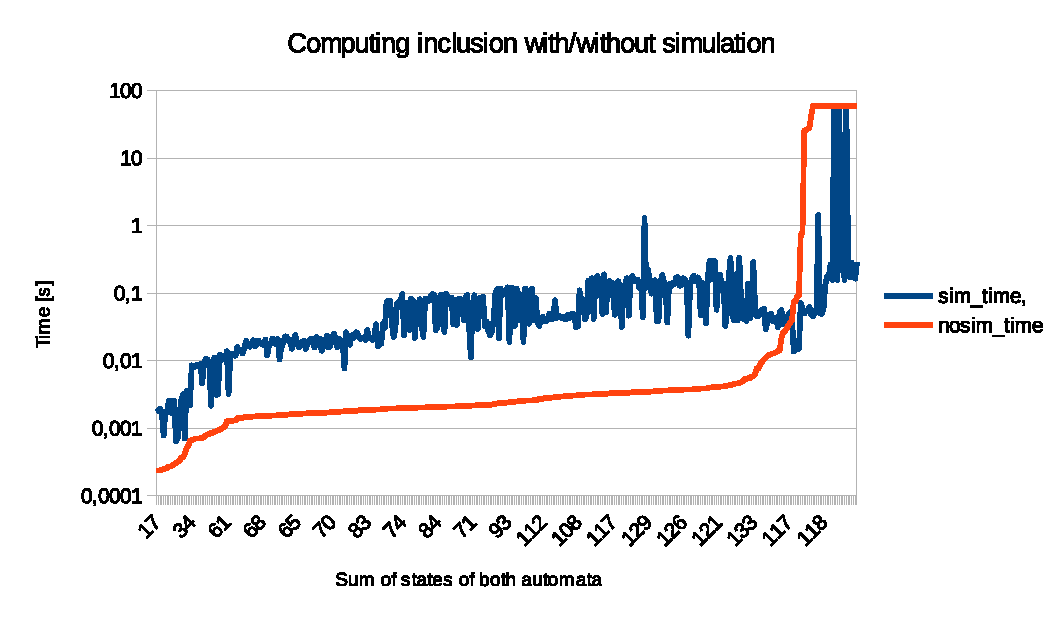
\includegraphics{g}
	\caption{}
	\label{fig:g}
\end{figure}

You can see that variant without simulation runs faster for most of the runs. It is because simulation is demanding per se and only prolong computation time of easily computed inclusions. Easily computed inclusions are those where we can refute inclusion right from start. On the other hand there is a region, where computation with simulation runs considerably slower than without simulation. You can see this region of previous plot in figure~\ref{fig:g_detail}.

\begin{figure}[h!]
	\centering
	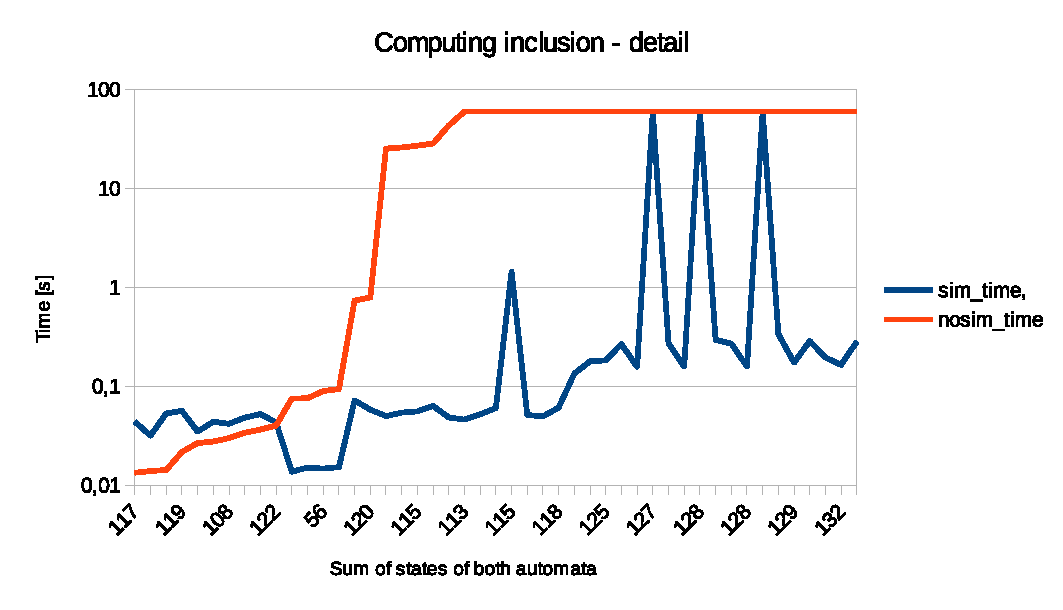
\includegraphics{g_detail}
	\caption{}
	\label{fig:g_detail}
\end{figure}

In this region we reduce some states and simulation runs comparably with previously described problems. This region is what we focus on and is main contribution of this work. For autotama with ~50 states run without simulation can run for ~4 minutes (in environment with disabled timeout) and gets worse with rising number of states. We are able to keep time of computation at ~1 second with simulation, for most cases. As you can see our run is terminated at timeout in some cases too, but in much lower number.

In next experiment we took automata with 110 - 170 states. You can see results of this experiment in figure \ref{fig:g_advanced}. Again you can see that for half cases computation without simulation is faster, but for second half our method  prevails. It still computes its results in 1 second while nosim run is cut off after 60 seconds. We were unable to check time of computation without simulation in these automata because it ran too long.

\begin{figure}[h]
	\centering
	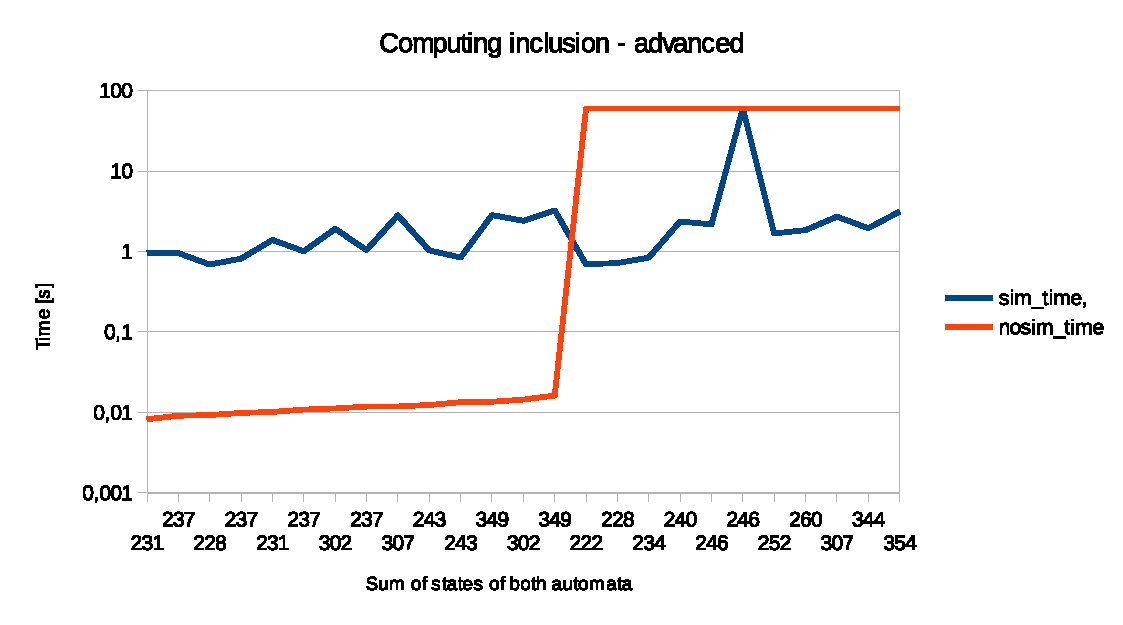
\includegraphics{g_advanced}
	\caption{}
	\label{fig:g_advanced}
\end{figure}

During performing of the test cases we found that currently implemented algorithm for computing simulation over explicitly represented NTA in VATA does not compute relation corresponding to the definition of simulation.
However, relation computed by VATA is subset of the correct simulation so it does not change correctness of checking language inclusion or reduction of NTA when simulation is exploited.

\section{Conclusion}
\label{sec:end}

This work describes implementation of a method for computing simulation over NTA and its implementation.
Our method takes NTA represented in semi-symbolic top-down way using MTBDD, it
turns it to explicit representation and compute downward simulation over it.

We implemented our method as module to VATA library using its infrastructure for manpilationg NTA.
The method has been evaluated on set of NTA and it has shown that our method is justifiable in some cases.
It ran 100x faster in these cases. On the other hand for most cases it runs slower than method without simulation because computing simulation is expensive and useless for some cases.
We also design and implemented enhanced algorithm for computing simulation and evaluated with following results. TODO
Another output of our work is that we found incorrectness of VATA algorithm for simulation computing.

Further research may be done in more efficient manipulation with MTBDD during translation to explicit representation or
extending it to bottom-up automata.
It is also possible to implement NTA reduction which uses computed simulation.
There is also room for further improvement of used algorithms and their efficient implementation.

\newpage
\appendix
\section{User guide}
\label{app:usage}

You can compile library if you satisfy prerequisites defined in file \textit{README} in project root folder. Compilation command is
\begin{verbatim}
$ make release
\end{verbatim}

When you have VATA compiled you can run simulation on file with command:
\begin{verbatim}
$ build/cli/vata -r bdd-td -o bdd=spec sim <AUTOMATON>
\end{verbatim}
This will run our code and will output simulation matrix. Simulation matrix $A$ where row index and column index are states. If value $A_{i,j}$ equals 1 it means that $i$ can be simulated by $j$, if 0 it means that $i$ cannot be simulated by $j$.

Automata for try-out are located in folder \texttt{automata/} or \texttt{tests/}.

If you want to run explicit simulation use command
\begin{verbatim}
$ build/cli/vata -r expl sim <AUTOMATON>
\end{verbatim}
Output is same as with run with our simulation.

You can compare these two results with python script
\begin{verbatim}
$ src/gal/compare_simulations.py <CORRECT_SIMULATION> <TEST_SIMULATION>
\end{verbatim}

To run inclusion with our simulation launch command
\begin{verbatim}
$ build/cli/vata -r bdd-td incl -t -o dir=down,rec=yes,sim=yes,bdd=spec <A1> <A2>
\end{verbatim}

If you want to run inclusion without our simulation run
\begin{verbatim}
$ build/cli/vata -r bdd-td incl -t -o dir=down,rec=yes <A1> <A2>
\end{verbatim}

For convenience we wrote two scripts that run previous two commands with timeout
\begin{verbatim}
$ src/gal/run_incl_nosim.sh <A1> <A2> 
$ src/gal/run_incl_sim.sh <A1> <A2>
\end{verbatim}

Script which will tests all given automata for inclusion in product
\begin{verbatim}
$ src/gal/test_inclusion.py <A1> [ <A2> [...]]
\end{verbatim}

\newpage
 
\bibliography{literatura}
\bibliographystyle{plain}
\end{document}
